\documentclass[a4paper]{article}

\usepackage[top=3cm, bottom=2cm, left=2cm, right=2cm]{geometry}
\usepackage{graphicx}
\usepackage{fancyhdr}
\usepackage{scrextend}
\usepackage[hidelinks]{hyperref}
\usepackage{textcomp}
\usepackage{tipa}
\usepackage{caption}
\usepackage{subcaption}
\usepackage{xcolor}

\graphicspath{ {./images/} }

\title{Homework 2 - Machine Learning: Weather Classification}
\author{Edoardo Piroli - 1711234}

\pagestyle{myheadings}
\pagestyle{fancy}
\fancyhf{}

\renewcommand{\headrulewidth}{0pt}
\renewcommand{\footrulewidth}{1pt}

\fancyfoot[C]{Report HW2 - Machine Learning}
\fancyfoot[R]{\thepage}

\begin{document}

\maketitle
\thispagestyle{empty}

\newpage
\tableofcontents
\thispagestyle{empty}
\newpage

\pagenumbering{arabic}

\section{Introduction}
\subsection{Assignment}
The assignment of the homework was to build an image classifier capable of assigning pictures to one of the following classes: \{\textit{RAINY}, \textit{HAZE}, \textit{SUNNY}, \textit{SNOWY}\}; based on how the weather was like at the moment of the picture's capture. In particular, the request was to address the former problem in 2 different ways: 
\begin{enumerate}
\item Applying transfer learning and fine-tuning on a pre-trained model;
\item Defining and training a CNN from scratch for this particular task.
\end{enumerate}
\subsection{Dataset}
The provided datasets\footnote{available here: \href{https://drive.google.com/drive/folders/1UzH28Q8xki8_DMYdDgHxi40-CJ800Kaq}{https://drive.google.com/drive/folders/1UzH28Q8xki8\textunderscore DMYdDgHxi40-CJ800Kaq}} are separated in several different archives and folders. I have chosen to use \textit{MWI-Dataset-1.1\textunderscore 2000} for training, \textit{MWI-Dataset-1.2.4} for testing and \textit{MWI-Dataset-1.2.5} for validation. All these datasets are perfectly balanced, in particular the training dataset is composed by 2000 pictures, 500 per class, while the validation and testing datasets are composed by 400 pictures(100 per class) each. 
\paragraph{Chosen resolution}
The pictures in the datasets don't share a common resolution, this is why I had to resize them in order to be able to train and test. 

In particular, I have chosen to use 299x299 as the pictures' resolution; I have tried other resolutions but this seemed to outperform the others(as expected since the chosen pre-trained model was originally trained on that resolution). I have tried 2 different approaches to resize the pictures:
\begin{enumerate}
\item \textbf{Padded}: Preserving the original aspect ratio, I have resized the longest side to 299, keeping constant the aspect ratio; i.e. proportionately resizing also the other side; and pasted the so-obtained picture on a black 299x299 square; basically adding some padding to the edges. As an example of this resizing process here is one sample picture:

\begin{figure} [h!]
\centering
\begin{subfigure}{0.5\textwidth}
  \centering
  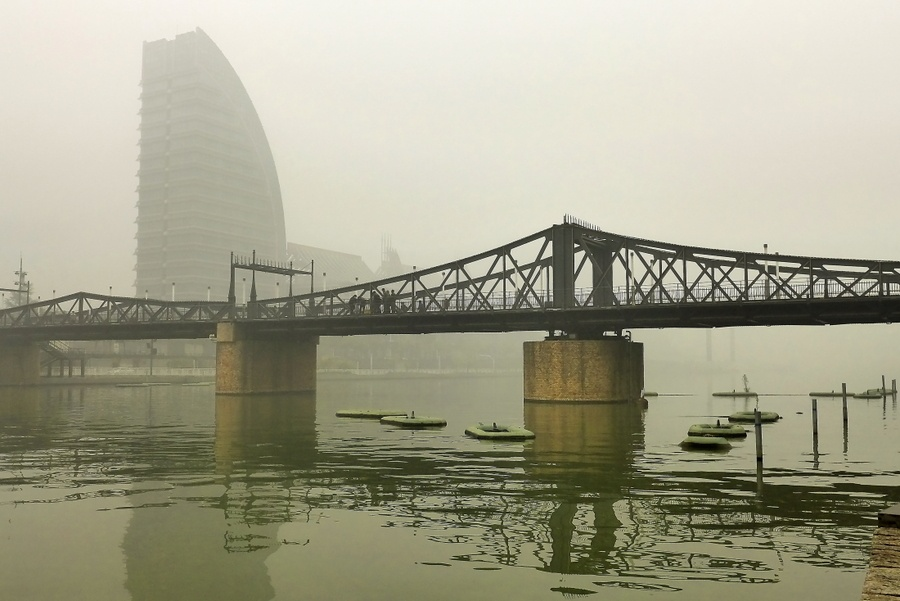
\includegraphics[width=0.99\textwidth]{HAZE-1-1-1_001_ORI.jpg}
  \caption{Original picture with resolution 900x601}
  \label{fig:sub1}
\end{subfigure}%
\begin{subfigure}{0.5\textwidth}
  \centering
  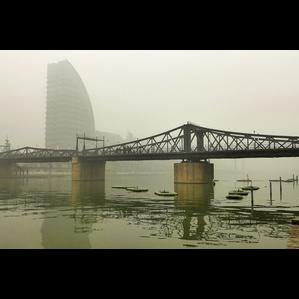
\includegraphics[width=0.99\textwidth]{HAZE-1-1-1_001_ORI_resized.jpg}
  \caption{Resized picture with resolution 299x299}
  \label{fig:sub2}
\end{subfigure}
\label{fig:test}
\end{figure}

\item \textbf{Non-Padded}: I've used the keras.preprocessing.image.ImageDataGenerator flow\textunderscore from\textunderscore directory method to resize the pictures.
\end{enumerate}

Although, differently from what I expected, the second, more classical, method of resizing performed better.
\section{Pre-trained Model}
After looking at the pre-trained models available \href{https://keras.io/applications}{\textcolor{blue}{\underline{here}}}, I have chosen to use the Xception model, characterised by a good ratio between size and accuracy.

The first pre-trained model that I tried is the following one, note that the xception model is completely frozen, i.e. its layers are not going to be modified during the backtracking phase: 
\begin{figure} [h!]
\centering
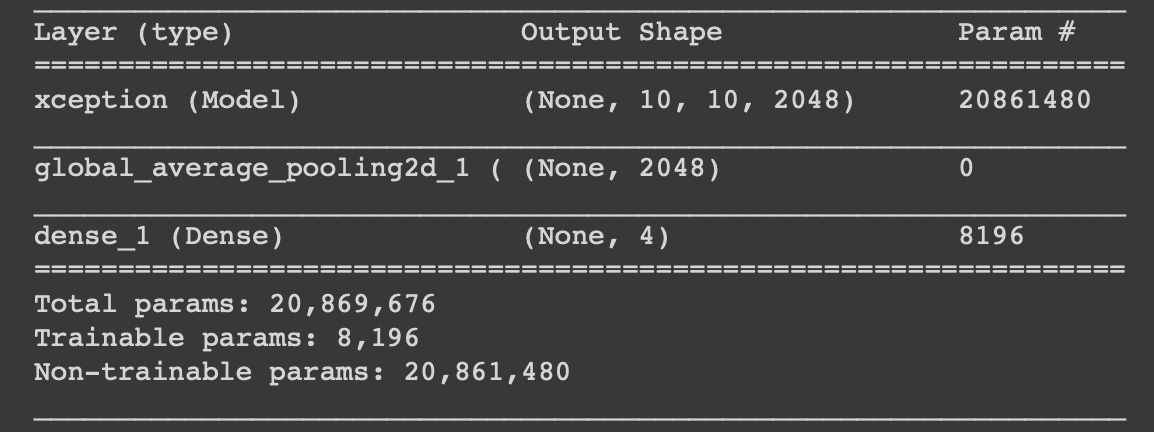
\includegraphics[width=\textwidth]{first_model.png}
\label{fig: first_model}
\end{figure}

Due to the small number of samples in the training dataset, this model performed poorly, clearly overfitting in less than 10 epochs:
\begin{figure} [h!]
\centering
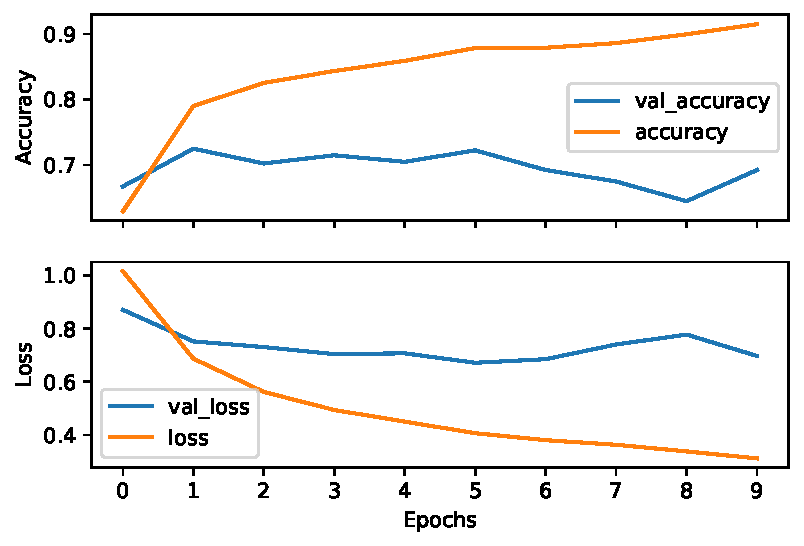
\includegraphics[width=\textwidth]{first_train.pdf}
\label{fig: first_train}
\end{figure}

\newpage
In order to alleviate this problem I have decided to try to add some dropout and regularization terms in the model, the final model which I obtained is the following one:

\begin{figure} [h!]
\centering
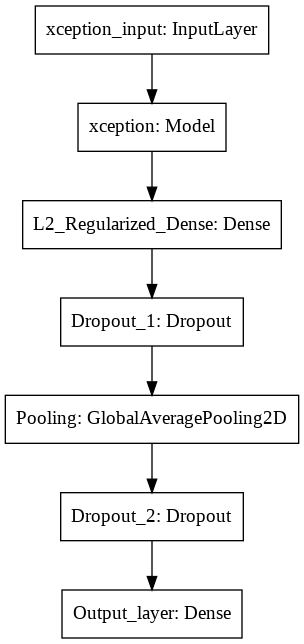
\includegraphics[width=0.5\textwidth]{final_model.png}
\label{fig: final_model}
\end{figure}

\subsection{Hyperparameters}
The hyperparameters of the pre-trained model are:
\begin{itemize}
\item \textbf{Dense size}: The size of the regularized dense layer;
\item \textbf{Regularization term}: The value for the kernel regularizer and the bias one;
\item \textbf{Dropout rate}: Shared among the 2 dropout layers;
\item \textbf{Activation Functions}: I have used 'softmax' for the output layer and 'relu' for the regularized dense layer;
\item \textbf{Optimization Function}: I have just used RMSProp;
\item \textbf{Learning rate}: The value used by RMSProp;
\item \textbf{Rho}: Other value used by RMSProp which I have set to 0.9, as suggested in the keras documentation;
\item \textbf{Epochs}: The number of epochs to train the models;
\item \textbf{Batch size}: I have used 50.
\end{itemize}
\subsection{GridSearch}
In order to try to optimize as much as possible the model I wanted to tune the hyperparameters performing a GridSearch, which in the end I carried out only partially due to time and computational power limitations.

In particular, I wanted to test the following values:
\begin{itemize}
\item \textbf{Dense size}: \{64, 128\};
\item \textbf{Regularization term}: \{0.001, 0.01\};
\item \textbf{Dropout rate}: \{0.3, 0.5\};
\item \textbf{Learning rate}: \{0.0001, 0.001\};
\item \textbf{Epochs}: I have used early stopping on the validation loss with patience=3.
\end{itemize}
\paragraph{Pre-trained model best hyperparameters:}
As expected, due to the great presence of overfitting, a higher value of the dropout rate and a smaller learning rate performed better.
\begin{center}
\begin{tabular}{|c|c|c|c|} 
 \hline
 \textbf{Dense size} & \textbf{Regularization term} & \textbf{Dropout rate} & \textbf{Learning rate} \\ 
 \hline
 128 & 0.001 & 0.5 & 0.0001 \\ 
 \hline
\end{tabular}
\end{center}
\subsection{Training tuned pre-trained model}
These are the plots of the training of the tuned pre-trained model:
\begin{figure} [h!]
\centering
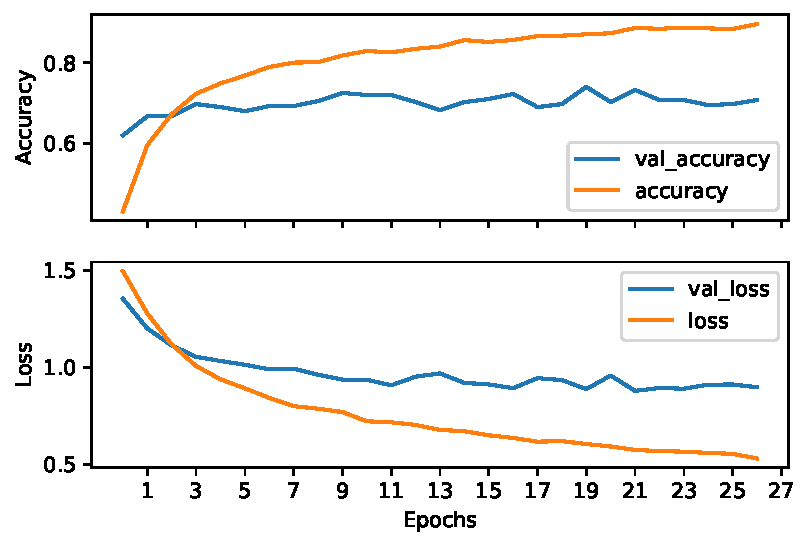
\includegraphics[width=0.8\textwidth]{pretrained_final_train.pdf}
\label{fig: pretrained_final_train}
\end{figure}

We can see that this model still overfits a lot but on a larger number of epochs w.r.t. the first model.
\newpage
\paragraph{Results of the final model:}
\begin{center}
\begin{tabular}{|c|c|c|} 
 \hline
 & \textbf{Accuracy} & \textbf{Loss}\\ 
 \hline
 \textbf{Training} & 0.886 & 0.574 \\
 \textbf{Validation} & 0.733 & 0.878 \\
 \textbf{Testing} & 0.715 & 0.983 \\
 \hline
\end{tabular}
\end{center}
\section{New Model}
I have chosen to implement the AlexNet model, as follows:
\begin{figure} [h!]
\centering
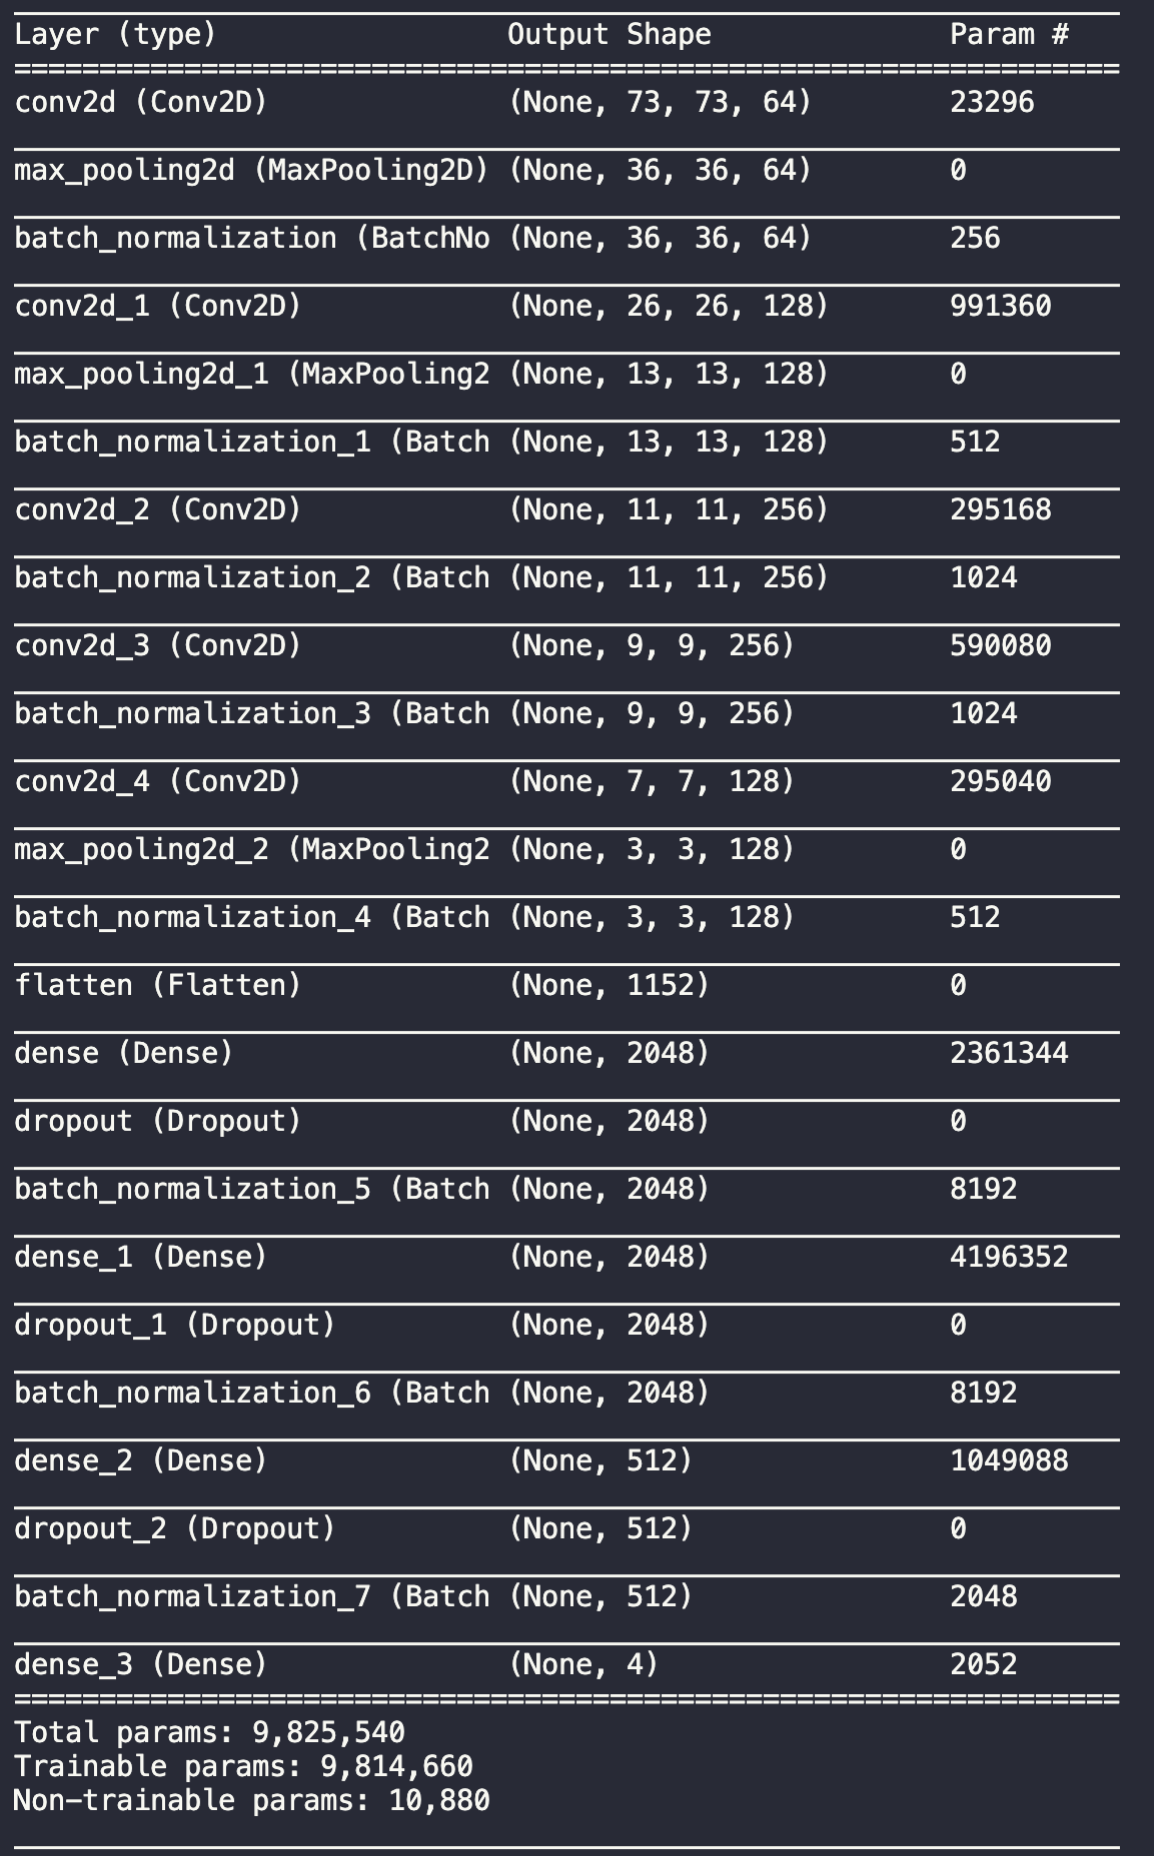
\includegraphics[width=0.73\textwidth]{new_model.png}
\label{fig: new_model}
\end{figure}
\newpage
\subsection{Training}
For this model, due to time limits, I have not run any hyperparameters tuning and this is one of the reasons why it performed extremely badly as we can see in the following plots:
\begin{figure} [h!]
\centering
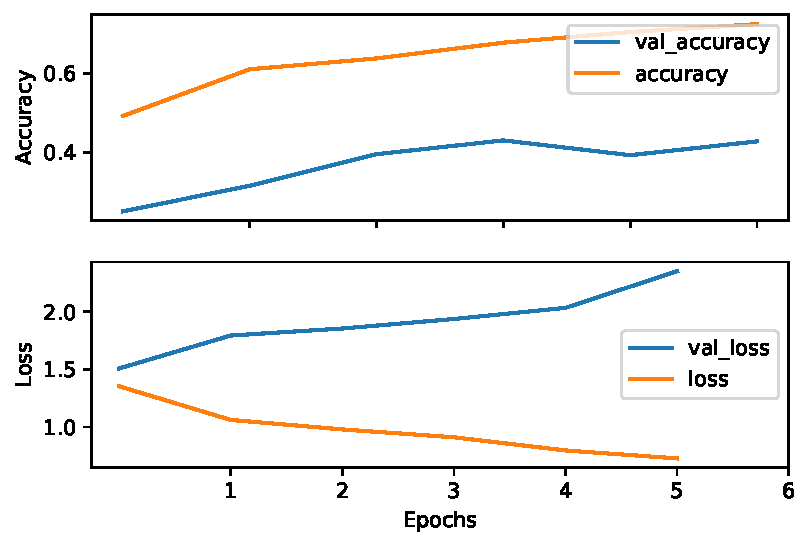
\includegraphics[width=\textwidth]{new_final_train.pdf}
\label{fig: new_final_train}
\end{figure}
\paragraph{Results of the final model:}
\begin{center}
\begin{tabular}{|c|c|c|} 
 \hline
 & \textbf{Accuracy} & \textbf{Loss}\\ 
 \hline
 \textbf{Training} & 0.492 & 1.354 \\
 \textbf{Validation} & 0.250 & 1.508 \\
 \textbf{Testing} & 0.433 & 2.267 \\
 \hline
\end{tabular}
\end{center}
\newpage
\section{Results}
\subsection{Comparison}
In the end, the pre-trained model, largely, outperformed the new one, this is mainly due to the following reasons:
\begin{enumerate}
\item I have spent more time and effort on the former model, and did not even manage to tune the hyperparameters of the latter one;
\item The pre-trained model has been trained for many epochs on a huge dataset of images and it can generate a well-refined set of features from each picture, this can represent a huge advantage when dealing with a niche task, like this one, with very few training samples.
\end{enumerate}

Obviously, I have submitted the pre-trained model.
\subsection{Proposed Improvements}
The results achieved can be largely improved, some ideas to do so are the following:
\begin{itemize}
\item Test other pre-trained models;
\item Improve the architecture of the model;
\item Train on more samples or perform data augmentation;
\item Test other hyperparameters' values or perform RandomSearch;
\item Test other resolutions.
\end{itemize}
\end{document}